\documentclass[12pt]{book}
\usepackage[utf8]{inputenc}
\usepackage{minted}
\usepackage{multirow}
\usepackage{listings}

\usepackage{amssymb,amsmath,amsthm,amsfonts}
\usepackage{calc}
\usepackage{graphicx}
\usepackage{subfigure}
\usepackage{indentfirst}
\usepackage{titlesec}
%\newcommand{\sectionbreak}{\clearpage}
\DeclareGraphicsExtensions{.bmp,.png,.pdf,.jpg}
\usepackage{gensymb}

\usepackage{url}
\usepackage{amsmath}
\usepackage{graphicx}
\graphicspath{{images/}}
\usepackage{parskip}
\usepackage{fancyhdr}
\usepackage{vmargin}
\setmarginsrb{2 cm}{2 cm}{2 cm}{2 cm}{1 cm}{1.5 cm}{1 cm}{1.5 cm}

\lstdefinelanguage{Marlowe}{%
  language     = Haskell,
  morekeywords = {Close, Pay, Assert, If, When, Let},
}
\lstdefinelanguage{Isabelle}{%
  language     = ML,
  morekeywords = {theory, imports, begin, end},
}

\definecolor{codegreen}{rgb}{0,0.6,0}
\definecolor{codegray}{rgb}{0.5,0.5,0.5}
\definecolor{codepurple}{rgb}{0.58,0,0.82}
\definecolor{backcolour}{rgb}{0.95,0.95,0.92}

\lstdefinestyle{Haskell-cardano}{
    backgroundcolor=\color{backcolour},   
    commentstyle=\color{codegreen},
    keywordstyle=\color{magenta},
    numberstyle=\tiny\color{codegray},
    stringstyle=\color{codepurple},
    basicstyle=\ttfamily\footnotesize,
    breakatwhitespace=false,         
    language=Haskell,
    breaklines=true,                 
    captionpos=b,                    
    keepspaces=true,                 
    numbers=none,                    
    numbersep=5pt,                  
    showspaces=false,                
    showstringspaces=false,
    showtabs=false,                  
    tabsize=2
}

\definecolor{isarblue}{HTML}{006699}
\definecolor{isargreen}{HTML}{009966}
\lstdefinelanguage{isabelle}{%
    keywords=[1]{type_synonym,datatype,fun,abbreviation,definition,proof,lemma,theorem, theory,corollary},
    keywordstyle=[1]\bfseries\color{isarblue},
    keywords=[2]{where,assumes,shows,and, imports, begin, end},
    keywordstyle=[2]\bfseries\color{isargreen},
    keywords=[3]{if,then,else,case,of,SOME,let,in,O},
    keywordstyle=[3]\color{isarblue},
}
\lstdefinestyle{Isabelle}{%
  language=isabelle,
  escapeinside={&}{&},
  columns=fixed,
  extendedchars,
  frame=single,
  basewidth={0.5em,0.45em},
  basicstyle=\ttfamily,
  mathescape,
}



\usepackage[spanish]{babel}
\usepackage[colorlinks=true, allcolors=blue]{hyperref}
\hypersetup{
    colorlinks=true,% make the links colored
}
\usepackage[nolist]{acronym}
\usepackage[table]{xcolor}
\usepackage{url}

%% Biblatex
% \usepackage[style=plain]{biblatex}
% \addbibresource{bibliografia.bib}

\begin{document}

\begin{titlepage}

    \title{     \textbf{Tesis de Grado \\ de Ingeniería en Informática}\\[2.5ex]
        \textit{Verificación de smart contracts en Marlowe\\ para la blockchain Cardano}}

    \author{
        \textbf{Director:} Dr.\ Ing. Mariano G. Beiró \\
        \texttt{mbeiro@fi.uba.ar}\\[2.5ex]
        \textbf{Co-director:} Phd. Simon Thompson (Kent University, IOHK) \\
        \texttt{S.J.Thompson@kent.ac.uk}
        \\[2.5ex]
        \textbf{Alumno:} Julián Ferres, \textit{(Padrón \#101.483)}                                \\
        \texttt{ jferres@fi.uba.ar }                                    \\[2.5ex]
        \normalsize{Facultad de Ingeniería, Universidad de Buenos Aires}        \\
    }
    \date{\today}

\end{titlepage}

\maketitle
\thispagestyle{empty}

\maketitle

{
    \hypersetup{linkcolor=black}
    \tableofcontents
}

%  Capítulos
%  1) Introducción (concepto de blockchain, aplicaciones, IOHK, Ada, Plutus) (8 a 10 páginas)
%  2) Escritura de contratos financieros en Marlowe para Cardano (15 a 20 páginas)
%     DONE a. El modelo UTXO
%     DONE b. Marlowe como DSL
%     Done c. El estándar ACTUS
%  3) Verificación de programas (12 a 15 páginas)
%     a. Concepto general, herramientas, metodologías
%     b. Isabelle
%  4) Desarrollo: verificación de contratos financieros usando Isabelle (30 páginas)
%     a. Escritura de contratos ACTUS para Cardano
%     b. sss
%     c. sss
%  5) Conclusión (3 páginas)
%  6) Bibliografía (4 páginas)
%  7) Apéndice (código)

%##########################
% INTRODUCCIÓN
%##########################

\chapter{Introducción}

\section{Cadena de bloques o Blockchain}
Las cadenas de bloques, conocidas en inglés como \textit{blockchains}, son estructuras de datos en las cuales la información se divide en conjuntos (bloques) que cuentan con información adicional relativa a bloques previos de la cadena.

Con esta organización relativa, y con ayuda de técnicas criptográficas, la información de un bloque solo puede ser alterada modificando todos los bloques posteriores.

Esta propiedad facilita su aplicación en un entorno distribuido, de manera tal que la cadena de bloques puede modelar una base de datos pública no relacional, que contenga un registro histórico irrefutable de información.

En la práctica esta técnica ha permitido la implementación de un registro contable o \textit{ledger} distribuido que soporta y garantiza la seguridad de transacciones y dinero digital.
El concepto de cadena de bloque fue aplicado por primera vez en 2009 como parte central de Bitcoin~\cite{nakamoto2008bitcoin}. En este trabajo, nos concentraremos en la cadena de bloques conocida como Cardano~\cite{cardano_website}~\cite{cardano_utxo_ledger}.

Con respecto a como se implementa en sistemas reales, una blockchain es un tipo de base de datos o libro mayor (`ledger') que se duplica y distribuye a todos los participantes dentro de la red de esa blockchain. Está formada por un conjunto de nodos interconectados que almacenan datos o elementos de valor en bloques. Estos bloques se verifican mediante transacciones y se vinculan entre sí mediante un orden cronológico en la cadena. Los detalles de estas transacciones están escritos de forma permanentemente en el bloque y no pueden modificarse.

Como una cadena de bloques almacena datos de manera descentralizada, es independiente de entidades de control centralizadas o intermediarios. Esto proporciona una mayor transparencia del almacenamiento de datos y su gestión. Una característica importante de blockchain es que almacena registros de forma inmutable, lo que significa que no se pueden cambiar, falsificar ni eliminar, ya que esto rompería la cadena de registros.

\begin{figure}
    \centering
    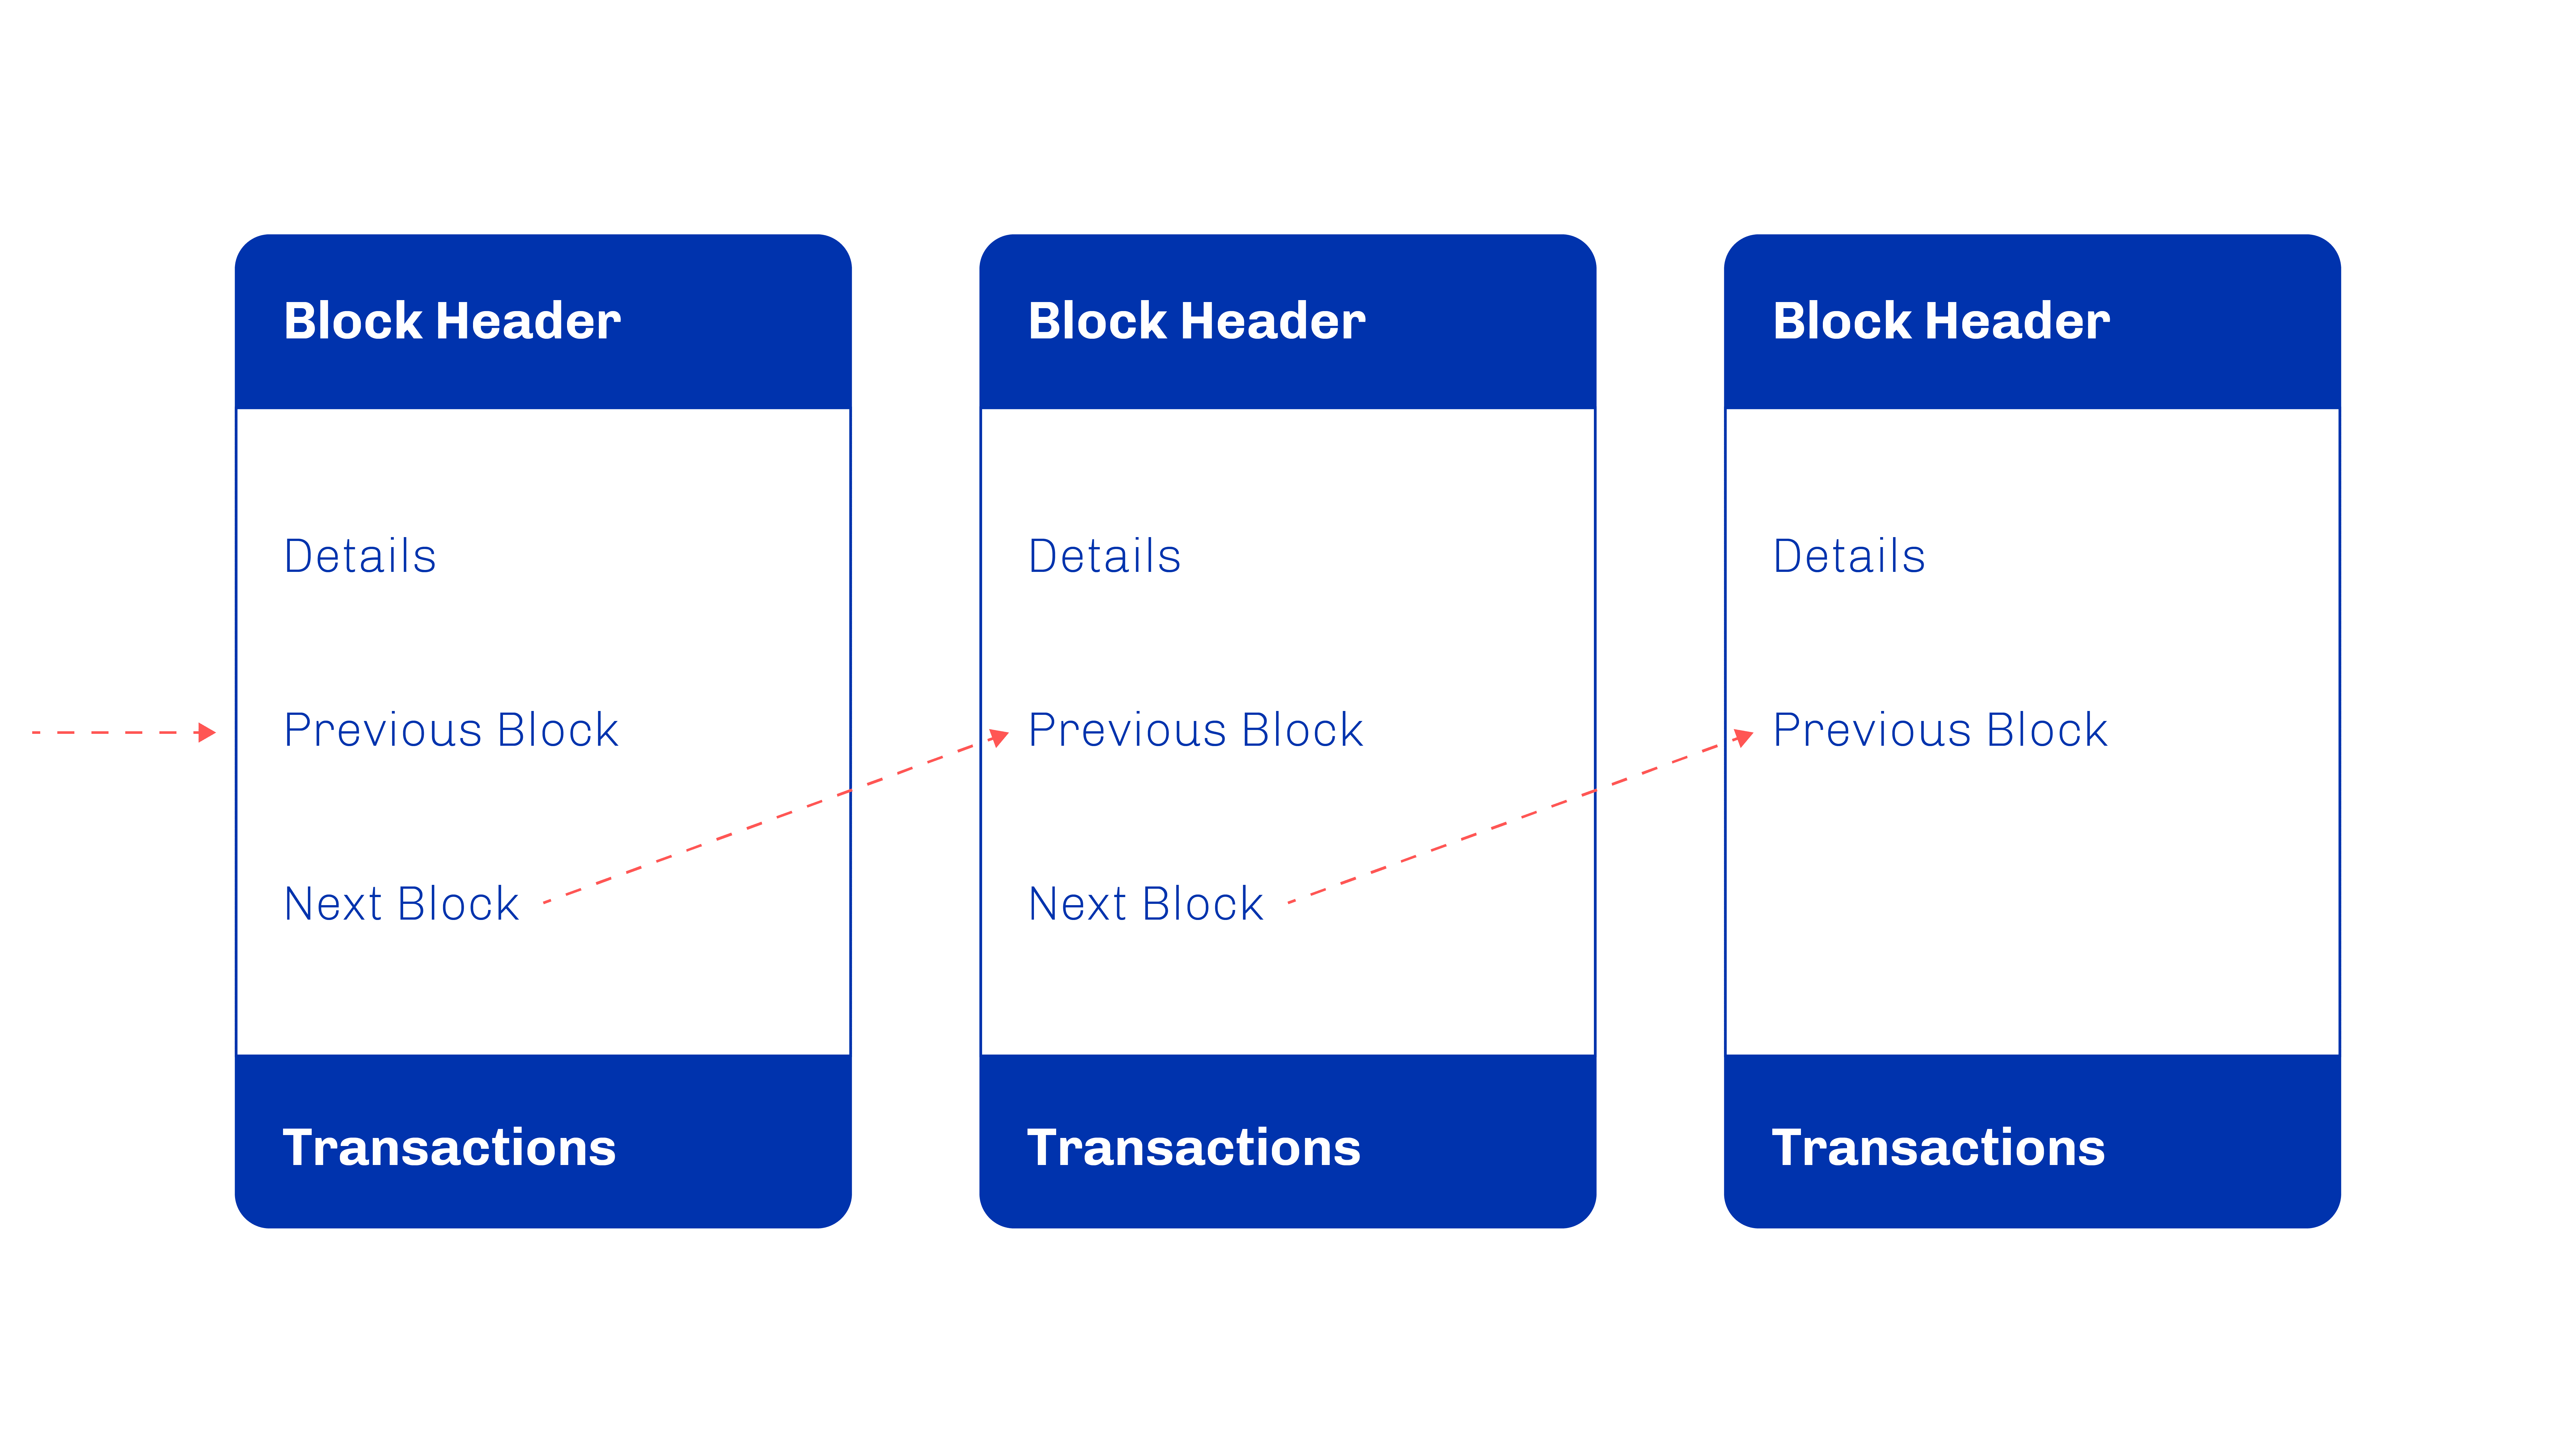
\includegraphics[width=0.9\textwidth]{Bloques.png}
    \caption{Representación simple de los datos contenidos en un bloque de la cadena}\label{fig:Bloques}
\end{figure}

Las cadenas de bloques no solo proporcionan una base de datos inmutable y segura, sino que también actúan como un entorno funcional para realizar transacciones de fondos, crear monedas digitales y procesar transacciones complejas mediante acuerdos digitales (`smart contracts').

% Tradicionalmente, un contrato se define como un acuerdo legalmente vinculante (por ejemplo, sobre un préstamo, venta, arrendamiento, etc). Un contrato inteligente permite forzar el cumplimiento de lo pactado en el mismo a través de una garantía asegurada por software, en la cual ninguna de las partes involucradas puede sabotear o alterar el contrato.

% De esta forma se puede renunciar a la toma de acciones legales por parte de un individuo, empresa o gobierno, y en su lugar optar por la ejecución de un programa, o contrato inteligente, para controlar la transferencia de fondos entre los participantes.
% Este objetivo se logra inmortalizando tanto el programa como su resultado en el ledger de la cadena de bloques subyacente al contrato, y garantizando así que todo el historial (incluido el estado actual del contrato) se registre de forma inmutable con un alto grado de fiabilidad. Desde la perspectiva del autor del contrato inteligente, la blockchain es un sistema de contabilidad distribuido, que realiza un seguimiento de quién posee una cantidad de un recurso virtual (Bitcoin, Ada, etc.) y cuándo los activos se transfieren de una entidad a otra.

Los propietarios de activos digitales se identifican por sus claves públicas, y pueden ser personas o máquinas.

\section{Smart contracts}

Un contrato inteligente o `smart contract' es un acuerdo digital automatizado, escrito en código, que trackea, verifica y ejecuta las transacciones vinculantes de un contrato entre varias partes. Las transacciones del contrato se ejecutan automáticamente mediante el código del smart contract cuando se cumplen las condiciones predeterminadas. Esencialmente, un contrato inteligente es un programa corto cuyas entradas y salidas son transacciones en una cadena de bloques.

Los smart contracts son autoejecutables y confiables y no requieren las acciones o la presencia de terceros. El código del contrato inteligente se almacena y distribuye a través de una red blockchain descentralizada, lo que lo hace transparente e irreversible.

En resumen, los contratos inteligentes son inmutables ya que no se pueden modificar, son distribuibles y a prueba de manipulaciones, rápidos y rentables, ya que no hay intermediarios, lo que ahorra dinero y tiempo, y es seguro gracias al cifrado del mismo.

Cardano presentará el soporte de contratos inteligentes en 2021. Como un entorno funcional, Cardano apoyará el desarrollo y la implementación de contratos inteligentes utilizando lenguajes de programación como:

\begin{itemize}
    \item \textbf{Plutus}: Una plataforma de desarrollo y ejecución de smart contracts especialmente diseñada. 
    Los contratos de Plutus consisten en partes que se ejecutan en la blockchain (`código on-chain') y partes que se ejecutan en la maquina del usuario (`código off-chain o de cliente').
    Plutus se basa en la investigación de lenguajes modernos para proporcionar un entorno de programación completo y seguro basado en Haskell, el lenguaje de programación funcional líder.
    
    \item \textbf{Marlowe}: Un lenguaje de dominio específico~\cite{fowler2010dsl} para escribir y ejecutar contratos financieros que permite construir contratos visualmente, así como en código más tradicional. Las instituciones financieras pueden usarlo para desarrollar e implementar instrumentos personalizados para sus clientes y usuarios. El propio lenguaje Marlowe está integrado tanto en JavaScript como en Haskell y ofrece una selección de editores según las preferencias y el conjunto de habilidades de los desarrolladores.
\end{itemize}


\section{Criptomonedas}

Una criptomoneda es un activo digital, que se almacena en el ledger y está diseñado para servir como medio de intercambio de bienes o servicios. Suelen ser popularmente llamadas `criptos'.

Los ledgers de blockchain son utilizados como tecnología subyacente para la creación de criptomonedas en un entorno descentralizado. Los protocolos de blockchain utilizan técnicas criptográficas rigurosas para permitir el minting (acuñación o creación) de criptomonedas, asegurar y verificar la propiedad de las mismas y los registros de movimiento de fondos. El precio de la criptomoneda no está controlado por un gobierno o una institución financiera centralizada. Se define por su valor, la correlación con las cifras del mundo real y está impulsado por la oferta y la demanda del mercado.

Las direcciones se utilizan al enviar pagos en criptomonedas. Son identificadores únicos y están representados por una cadena de números y letras que se obtienen de las claves públicas del usuario.

\section{Cardano}

Cardano~\cite{cardano_docs} es una plataforma blockchain de tipo `proof-of-stake' (prueba de participación)
\footnote{Definiciones sobre PoS se encuentran en los sitios web de \href{https://ethereum.org/en/developers/docs/consensus-mechanisms/pos/}{Ethereum} y \href{https://www.coinbase.com/es/learn/crypto-basics/what-is-proof-of-work-or-proof-of-stake}{Coinbase}}
descentralizada de tercera generación y el hogar de la criptomoneda ada. Es la primera plataforma de cadena de bloques que evoluciona a partir de una filosofía científica y un enfoque impulsado por la investigación.

\begin{figure}[H]
    \centering
    
\includegraphics[width=0.5\textwidth]{Cardano_logo.png}
    \caption{Logo de la cadena de bloques Cardano}\label{fig:Cardano_logo}
\end{figure}


La plataforma Cardano ha sido diseñada desde cero y verificada por una combinación de ingenieros y expertos académicos en los campos de blockchain y criptografía.
Tiene un fuerte enfoque en la sostenibilidad, la escalabilidad y la transparencia. 
Es un proyecto totalmente de código abierto que tiene como objetivo ofrecer una infraestructura inclusiva, justa y resistente para aplicaciones financieras y sociales a escala global. 

Uno de sus principales objetivos es brindar servicios financieros confiables y seguros a aquellas personas que actualmente no tienen acceso.

Cardano ha sido diseñado con la seguridad como uno de sus principios fundamentales. 

Está escrito en Haskell, un lenguaje de programación funcional. 
En un lenguaje funcional como Haskell, se fomenta la construcción de su sistema usando funciones puras, lo que conduce a un diseño en el que los componentes se pueden probar convenientemente de forma aislada. 
Además, las funciones avanzadas de Haskell nos permiten emplear una amplia gama de métodos potentes para garantizar la corrección del código, como basar la implementación en especificaciones formales y ejecutables, pruebas exhaustivas basadas en propiedades y ejecutar pruebas en simulación.

Cardano está desarrollando una plataforma de `smart contracts' que busca ofrecer funciones más avanzadas que cualquier protocolo desarrollado anteriormente, y servirá como una plataforma estable y segura para el desarrollo de dApps de nivel empresarial.

\subsection{Ada como criptomoneda de Cardano}


Cada ledger de blockchain tiene su criptomoneda subyacente o moneda nativa. Ada es la moneda nativa o principal en Cardano. Esto significa que ada es la principal unidad de pago en Cardano; se acepta como pago de cuotas, para realizar depósitos, y también es la única moneda en la que se distribuyen las recompensas.

Lovelace es la denominación más pequeña de ada. $\boxed{ 1 \text{ ada} = 1.000.000 \text{ lovelaces}}$. Ada tiene seis decimales, lo que la hace fácilmente divisible en fracciones más pequeñas.

\subsubsection{Tokens nativos}

Cardano también admite la creación de tokens nativos: activos digitales que se crean para fines específicos. Esto significa que los usuarios, desarrolladores y empresas pueden usar la cadena de bloques de Cardano para crear tokens que representen una huella de valor (ya sea definida por la comunidad, el estado del mercado o la entidad autónoma). Un token puede ser fungible (intercambiable) o no fungible\footnote{Ampliamente conocido por su acrónimo en inglés NFT} (único) y actuar como unidad de pago, recompensa, activo comercial o contenedor de información.


% Dada la importancia de los smart contracts para respaldar actividades en todos los sectores de la industria, incluyendo cadenas de abastecimiento, finanzas, servicios legales y médicos, existe una fuerte demanda de verificación y técnicas de validación sobre los mismos. Sin embargo, la gran mayoría de los contratos inteligentes carecen de cualquier tipo de especificación formal, que es esencial para establecer que el mismo es correcto.

% En este trabajo nos proponemos estudiar la verificación a bajo nivel de un grupo específico de contratos financieros definidos en el estándar ACTUS\footnote{\href{https://www.actusfrf.org/}{https://www.actusfrf.org/}}, en particular para la cadena de bloques \textit{Cardano}\footnote{\href{https://cardano.org/}{https://cardano.org/}}.


\subsection{Proof of stake}

Proof of stake (PoS o Prueba de participación) es un tipo de protocolo de consenso que utiliza la cantidad de participación (o valor) mantenida en el sistema para determinar el consenso.

En esencia, un protocolo de consenso es lo que controla las leyes y los parámetros que rigen el comportamiento de las cadenas de bloques. El consenso puede resumirse como un conjunto de reglas a las que se adhiere cada participante de la red.

Dado que las blockchains no están controladas por ninguna autoridad central única, en su lugar se utiliza un protocolo de consenso para permitir que los participantes de la red distribuida acuerden el historial de la red reflejada en la cadena de bloques, para llegar a un consenso sobre lo que ha sucedido y continuar desde una sola fuente de `verdad'.

Cardano se basa en el protocolo de consenso PoS llamado Ouroboros~\cite{pof_ouroboros}, el primer protocolo de consenso de blockchain que se desarrolla a través de una investigación revisada por pares. En el corazón del protocolo se encuentran los `stake pools' (grupos de participación), nodos servidores confiables administrados por un operador de `stake pools' en los que los titulares de ada pueden delegar su participación. Los `stake pools' se utilizan para garantizar que todos puedan participar en el protocolo, independientemente de la experiencia técnica o la disponibilidad para mantener un nodo en funcionamiento.

\subsubsection{Proof of stake vs. Proof of work}

Por el contrario, el protocolo conocido como `Proof of work' (PoW) o prueba de trabajo es un mecanismo síncrono que anima a los mineros a competir para ser los primeros en resolver cualquier problema dentro del bloque. Se utiliza un sistema de recompensas para incentivar esta resolución de problemas. Sin embargo, este enfoque acarrea una gran desventaja, con un mayor uso de electricidad y períodos de tiempo más largos para resolver problemas dentro de la cadena. Estos factores pueden ralentizar la red significativamente y significativamente más costosa de mantener.

\subsubsection{Características del protocolo proof of stake}

Una de las características clave de PoS es que a medida que aumenta el valor del usuario, también aumenta la oportunidad de mantener el ledger.

Esto significa una mayor probabilidad de producir nuevos bloques que se pueden agregar a la cadena de bloques. El creador de un nuevo bloque se elige en función de una combinación de selección aleatoria y una medida de su participación o riqueza. Dentro de la cadena se produce una especie de elección de líder. Cabe aclarar que dentro de un protocolo de prueba de participación, los participantes acumulan las tarifas de transacción, lo que aumenta su riqueza a medida que avanzan. Este enfoque fomenta el crecimiento constante y estable de la blockchain y reduce los casos de transacciones estancadas que pueden impedir el crecimiento de la misma.

\subsubsection{Principales ventajas de Proof of Stake por sobre Proof of Work}

\begin{itemize}
    \item Se incorporan rigurosos protocolos de seguridad en un protocolo PoS.
    \item Centralización reducida: el riesgo de centralización se reduce al emitir sanciones por prácticas egoístas dentro de la red
    \item Eficiencia energética: el consumo de energía es extremadamente eficiente ya que se necesita una cantidad menor de electricidad, así como recursos de hardware, para producir y ejecutar la cadena de bloques.
    \item Eficiencia de costos: las monedas PoS son mucho más rentables que las que operan en los protocolos PoW.
\end{itemize}


%#########################################################################
% ESCRITURA DE CONTRATOS FINANCIEROS EN MARLOWE PARA CARDANO
%#########################################################################


\chapter{Escritura de contratos financieros en Marlowe para Cardano}

\section{El modelo UTXO} % TODO: No hay bib del libro de plutus, considero escribir la entrada por mi mismo

Para poder entender la estructura de los contratos en Cardano, es importante tener comprensión de como se lleva a cabo la contabilidad en la misma.
Tradicionalmente, pensamos en las transferencias de dinero entre dos cuentas bancarias, o quizás direcciones de Internet en el caso de la moneda digital.

La plataforma Cardano, asi como otras plataformas de criptomonedas como Bitcoin, utilizan en su lugar un enfoque contable conocido como UTXO~\cite{cardano_utxo_ledger} (Unspent transaction output, o `Salida de transacción no utilizadas').

El modelo UTXO~\cite{Translating_and_Unifying_UTXO-based}\cite{UTxO_Lars} documenta el flujo de dinero no de cuenta a cuenta, sino de \textbf{transacción a transacción}. Cada transacción tiene entradas (de dónde proviene el dinero que se gasta) y salidas (hacia donde se dirige este dinero).

Consideremos el gráfico de flujo de dinero en la figura~\ref{fig:UTXO_Funds_Flow_Example}. Las lineas negras representan outputs no gastados de las transacciones, y las lineas rojas representan dichos outputs siendo utilizados como inputs de transacciones posteriores.

Las cajas sin etiquetas representan una transacción (que contiene varios inputs y outputs). Los certificados azules denotan los outputs no gastados disponibles en nuestra ilustración.

Al comienzo del gráfico de flujo, Alice tiene 100 Ada en `outputs sin utilizar' previos al comienzo de nuestro análisis. Este dinero proviene de una o más transacciones pasadas, que exceden el alcance del gráfico. Simplificamos el mismo con una simple caja (etiquetada con su nombre y el dinero correspondiente).

Dicha caja tiene dos lineas negras (outputs) saliendo de ella, siendo la suma del valor de las mismas 100 Ada:

\begin{itemize}
    \item Un output de 58 Ada permanece sin ser utilizado y es parte de los outputs sin utilizar al final del análisis.
    \item Un output de 42 Ada se utiliza como parte de la nueva transacción.
\end{itemize}

Por su parte, Bob tiene 10 Ada de previos outputs sin utilizar. Los utiliza a todos en la nueva transacción. La transacción que ilustramos tiene dos inputs: 42 de Alice y 10 de Bob. La misma también tiene dos outputs: 2 para Bob y 50 para Charlie.

Vemos también que Charlie tiene 52 Ada provenientes de outputs previos a nuestro gráfico, totalizando 102 Ada que puede utilizar en transacciones futuras. Bob termina con solo un output de 2 Ada, y Alice con un total de 58 Ada.

\begin{figure}
    \centering
    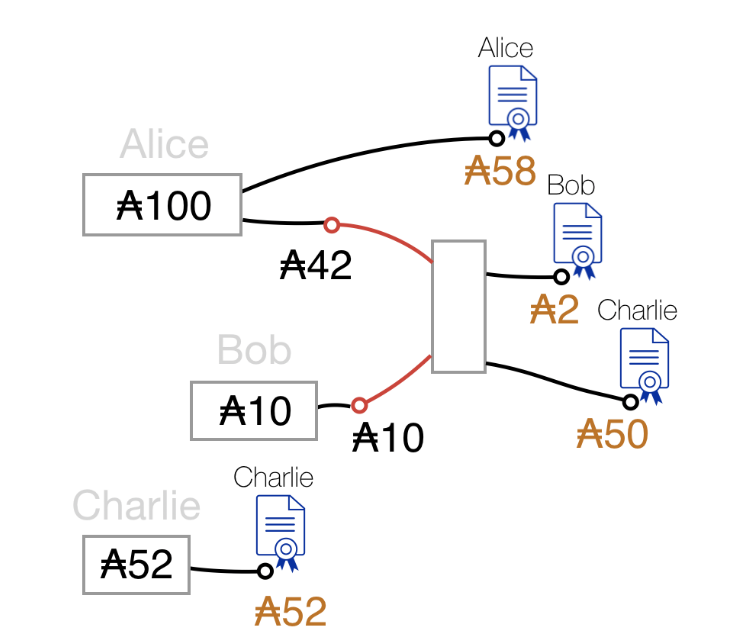
\includegraphics[width=0.7\textwidth]{UTXO_Funds_Flow_Example.png}
    \caption{Flujo de dinero en el modelo UTXO}\label{fig:UTXO_Funds_Flow_Example}
\end{figure}

El modelo anterior muestra estrictamente el flujo de dinero entre varios participantes. En esta versión simplificada, por ejemplo, las transacciones ilustradas no pagan comisiones. Sin embargo, en este modelo simplificado, vemos que los outputs deben gastarse en su totalidad. Es decir, un registro de un output no gastado no puede ser modificado (esta acción se adecua mas a los modelos contables basados en cuentas), solo podría utilizarse de forma completa.

Para mantener la integridad de la contabilidad, las nuevas transacciones debe tener todas las outputs no gastados (totalizando la cantidad correcta de outputs no gastados) utilizados como entrada.

En nuestro ejemplo anterior, la nueva transacción elimina (utilizándolas como entrada) a los outputs no gastados de valor 42 de Alice y 10 de Bob, para un total de 52 Ada. Esto implica que la transacción esta obligada a totalizar 52 Ada como outputs sin gastar (que de hecho cumple, con 2 para Bob y 50 para Charlie).

Un aspecto a destacar es que Bob tiene un `unspent output' como entrada y uno como salida. Esto se podría interpretar como un `cambio' (de 2 Ada) para esta transacción. Dicho concepto es similar al que utilizamos en el día a día al realizar pagos en efectivo: Si un producto cuesta \$98 y tenemos un billete de \$100, no podemos fraccionar dicho billete. Tenemos que pagar con todo el billete y recibir \$2 de cambio.

Dado que no existe una forma real de gastar parte de un `unspent output', así es como el modelo UTXO trata el gasto parcial: agregando una salida de `cambio'.

Cabe destacar que este modelo contable hace que sea conveniente distribuir el flujo de efectivo de varios contribuyentes a varios destinatarios haciendo que el mismo fluya hacia un fondo común, en este caso, la transacción, antes de enviarse a los beneficiarios finales. Esto representa, en un sentido muy general, el objetivo de los `smart contracts' o contratos inteligentes.

Veamos más formalmente lo que sucede durante una transacción en el modelo UTXO.\@Para el modelo de transacciones basico que analizaremos, podemos referirnos a las definiciones en la figura~\ref{fig:Basic_UTXO_definitions}:


\begin{figure}[H]
    \centering
    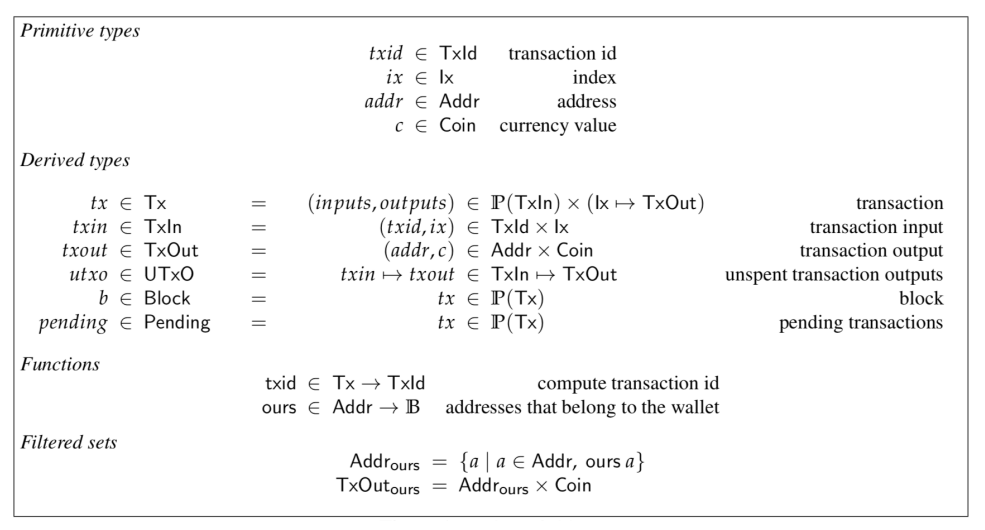
\includegraphics[width=0.9\textwidth]{Basic_UTXO_Definitions.png}
    \caption{Definiciones básicas en el modelo UTXO}\label{fig:Basic_UTXO_definitions}
\end{figure}

Antes de analizar la estructura de las transacciones, haremos un pequeño repaso sobre como la contabilidad se lleva a cabo en el `libro mayor' o ledger. El registro que contiene la información sobre el ledger es llamado \texttt{UTXO}. Este registro es un map finito, donde la key o clave is un par formado por el id de la transaccion y un indice, \texttt{TxIn = TxId * Ix}. El id de la transacción puede ser calculado en base a una transacción completada para procesar, y es un identificador único de la transacción.

El índice \texttt{Ix} es necesario debido a que puede haber mas de un output en dicha transacción, y cada uno de los mismos tiene que tener un identificador único dentro de el conjunto de `outputs' dentro de una transacción.

Los valores o values en el mapa son pares formados por un `coin value' y una direccion, y el tipo de los mismos es \texttt{TxOut = Addr * Coin}. Cabe destacar que las direcciones de los usuarios son siempre claves públicas, y los fondos en ellas pertenecen a la entidad que puede probar que posee la clave privada correspondiente. Las direcciones de `script' (smart contract o contrato inteligente) se comportan de manera ligeramente distinta, debido a que no tienen un dueño directo.

Para poder comprender la escturctura de la transacción en sí, analicemos primero los `outpus'. Una transacción puede distribuir el dinero que está gastando a varias direcciones diferentes. Los outputs, (valores de tipo \texttt{TxOut}) se almacenan en una transacción como valores en un mapa finito.
Las claves del mapa son indices únicos dentro del contexto del mapa, de manera tal que la combinación del id de la transacción y dicho indice identifica de forma global a dicho output.
En el modelo UTXO, se relaciona a los valores de salida con las entradas de las cuales provienen, por medio de este identificador global compuesto.


Los inputs, cuyo orden no es relevante, son un conjunto y no una lista. Los elementos de este conjunto no contienen ni el valor de la moneda a gastar, ni la dirección de donde proviene el dinero. Esta es la principal distinción entre el modelo contrable tradicional y el UTXO:\@el dinero que se gasta solo referencia a los outputs no gastadas de transacciones previamente procesadas en el `ledger' que reside actualmente en la blockchain. Cada elemento del mencionado set de inputs es un par formado por el id de la transacción y un indice que, como se explicó anteriormente, identifica de forma única el output no gastado en la UTXO.\@

Procesar una transacción implica actualizar el \texttt{UTXO} en el ledger de manera tal que los fondos gastados por la transacción que se está procesando estén disponibles para que los gasten los propietarios de las direcciones de las salidas de la transacción. Es decir, todas las entradas correspondientes a inputs de la transacción procesada se eliminan del ledger \texttt{UTXO}.

Adicionalmente, todos los valores de \texttt{TxOut} en el mapa finito de las salidas de la transacción se agregan a la \texttt{UTXO}, con la clave del mapa finito que consiste en el id de la transacción que se procesa, y el valor del índice es el mismo que en el mapa finito de salidas de esta transacción. Es decir, si \texttt{tx} contiene un par formado por el conjunto de entrada y el mapa de salidas \texttt{(ins, outs)} con id \texttt{id}, y \texttt{ix |-> (a, c)} es una entrada de \texttt{outs}, la \texttt{UTXO} va a tener la entrada \texttt{(id, ix) |-> (a, c)} agregada. En este párrafo, utilizamos la notación \texttt{k |-> v} para referirnos a una entrada del mapa finito con clave \texttt{k} y valor \texttt{v}.

Veamos como se refleja dicha actualización del ledger en terminos de notación matemática (que puede ser reflejada en código con relativa facilidad). Las siguientes son tres formas de filtrar el mapa finito de \texttt{UTXO}. El primero filtra dicho mapa mediante un subconjunto \texttt{ins} de las claves. El segundo filtro obtiene el complemento del resultado del primer filtro (en otras palabras, todas las entradas de la \texttt{UTXO} que no son indexadas por claves en la lista de inputs). El tercero filtra el mapa mediante los valores.

\begin{center}
    \begin{tabular}{ r @{} c @{} l r }
        \texttt{ins} $\lhd$ \texttt{utxo} &\ =\ \ & $\{ i \mapsto o\ |\ i \mapsto o \in utxo,\ i \in ins \}$ & restricción de dominio \\
        \texttt{ins} $\ntriangleleft$ \texttt{utxo} &\ =\ \ & $\{ i \mapsto o\ |\ i \mapsto o \in utxo,\ i \notin ins \}$ & exclusión de dominio \\
        \texttt{utxo} $\rhd$ \texttt{outs} &\ =\ \ & $\{ i \mapsto o\ |\ i \mapsto o \in utxo,\ o \in outs \}$& restricción de rango
    \end{tabular}
\end{center}

Utilizaremos la notación introducida para procesar una nueva transacción. En otras palabras, eliminar los ouputs no gastados correspondientes y construir un nuevo conjunto de outputs que serán agregados al \texttt{UTXO} (como se describió anteriormente). Los outputs a agregar serían computados de la siguiente manera:

% \begin{equation}
%     $ \text{txins} \in \mathbb{P}(\text{Tx}) \rightarrow \mathbb{P}(\text{TxIn}) $ &&
%     hola
% \end{equation}

\begin{center}
    \begin{tabular}{|r c l|}
        \hline &&\\
        $\text{txins}$ & $\in$ & $\mathbb{P}(\text{Tx}) \rightarrow \mathbb{P}(\text{TxIn})$ \\&&\\

        $\text{txins } txs$ & = & $\bigcup \{ inputs\ |\ (inputs, \_ ) \in txs$\} \\&&\\

        $\text{txouts}$ & $\in$ & $\mathbb{P}(\text{Tx}) \rightarrow \text{UTXO}$ \\&&\\

        $\text{txouts } txs$ & = &
            $\left\{
                \begin{array}{l|lcl}
                    & tx & \in & txs \\
                    (\text{txid } tx, ix) \mapsto txout & (\_, outputs) & = & tx \\
                    & ix \mapsto txout & \in & outputs \\
                \end{array}
            \right\} $ \\&&\\
        \hline
    \end{tabular}
\end{center}

Usando esta notación, podemos definir la actualización del \texttt{UTXO}, debido a la transacción \texttt{tx} como:

\[ (\text{txins } tx\ntriangleleft\ utxo) \cup\text{outs } tx \]

Hay que tener en cuenta que se debe realizar un cálculo expícito de la cantidad total de Aca en las salidas y el total de Ada en todas las entradas de una transacción como parte de la validación de la transacción. También podría haber outputs en una transacción sin inputs correspondientes; estos se deben a la recolección de recompensas.

Ahora, para validar una transacción, se realiza una serie de cálculos que involucran el Ada en la misma y el Ada en otras cuentas del ledger, para asegurarse de que no se crea ni se destruye dinero. Esto se conoce como `propiedad contable generalizada'. El modelo contable UTXO brinda protección integrada contra el `doble gasto' de un output determinado.

Esta protección inherente, junto con la aplicación de la propiedad contable generalizada, asegura que no se permita que ocurra ningún gasto deshonesto. Esta es una propiedad crucial del sistema contable del ledger de Cardano, en particular porque existe una cantidad fija de Ada que nunca puede cambiar.

Para finalizar, hay que tener en cuenta que una transacción incluye una gran cantidad de datos adicionales, como testigos, certificados, y scripts juntos con sus hashes. En esta sección no hemos entrado en los detalles de los tipos y cálculos específicos utilizados en la implementación del ledger de Cardano. Sin embargo, abarcamos suficiente información como para poder entender que sucede detras de escena cuando se genera una transacción en la blockchain.


\section{Marlowe como DSL}
Marlowe~\cite{implementing_financial_contracts_on_blockchain}~\cite{standardized_crypto_loans} es un lenguaje pequeño, con pocas sentencias soportadas que, para cada contrato, describen el comportamiento que involucra un conjunto fijo y finito de roles.

Marlowe está diseñado para crear bloques para contratos financieros: pagos o depósitos de las partes, elecciones e información del mundo real. Cuando se ejecuta un contrato, los roles que implica son satisfechos por los participantes, que son identidades en la cadena de bloques. Cada rol está representado por un token en la cadena y los roles se pueden transferir durante la ejecución del contrato, lo que significa que esencialmente se pueden intercambiar.

Los contratos se pueden construir reuniendo una pequeña cantidad de estas sentencias que, en combinación, se pueden usar para describir y modelar muchos tipos diferentes de contratos financieros. Algunos ejemplos incluyen un contrato que puede realizar un pago a un rol o a una clave pública, un contrato que puede esperar una acción por parte de uno de los roles, como un depósito de moneda, o una elección entre un conjunto de opciones.

En particular, un contrato no puede esperar indefinidamente una acción: si no se ha realizado en un tiempo determinado (conocido como \textit{timeout}), el mismo continuará con un comportamiento alternativo, por ejemplo, reembolsar los fondos en el contrato.

Los contratos de Marlowe pueden ramificarse en función de alternativas y tienen una vida finita, al final de la cual el dinero restante retenido por el mismo se devuelve a los participantes. Esta característica garantiza que el dinero no se puede bloquear para siempre en un contrato. Dependiendo del estado actual de un contrato, puede elegir entre dos cursos de acción alternativos, que son en sí mismos contratos. Cuando no se requieran más acciones, el contrato se cerrará y se reembolsará cualquier moneda restante en el contrato.

\subsection{Contratos en Marlowe}
Un contrato en Marlowe se obtiene combinando una pequeña cantidad de sentencias o \textit{building blocks}. Las mismas pueden llegar a describir muchos tipos de contratos financieros, como hacer un pago, hacer una observación, esperar hasta que cierta condición se cumpla, etc. Luego, el contrato se ejecuta en una cadena de bloques, como Cardano, e interactúa con el mundo exterior.

Marlowe, en sí mismo, está embebido en Haskell y se modela como una colección de tipos de datos algebraicos en Haskell~\cite{Algebraic_data_type}, con contratos definidos por el tipo de contrato:

\begin{lstlisting}[language=Marlowe]
data Contract = Close
              | Pay Party Payee Token Value Contract
              | If Observation Contract Contract
              | When [Case] Timeout Contract
              | Let ValueId Value Contract
              | Assert Observation Contract
\end{lstlisting}

Marlowe tiene seis maneras de construir contratos. Cinco de esos métodos ---
\texttt{Pay}, \texttt{Let}, \texttt{If}, \texttt{When}, and \texttt{Assert} --- construyen un contrato complejo a partir de contratos más simples, y el ultimo método, \texttt{Close} es un contrato simple. En cada paso de la ejecución, además de modificar el estado y proceder hacia un nuevo contrato, podrían generarse pagos y advertencias (\textit{warnings}).

Antes de describir los métodos exhaustivamente, es útil conocer la definición de valores, observaciones y acciones:

\begin{enumerate}
    \item \textbf{Valores}: Incluyen cantidades que cambian con el tiempo, tales como: el \textit{slot interval} o `intervalo actual', el balance de cierto token en una cuenta o elecciones que se han realizado (conocidas como \textit{valores volátiles}). Los valores pueden ser combinados usando operaciones como suma, resta, negación, etc. Los mismos pueden ser valores condicionales o una observación.

    \item \textbf{Observaciones}: Valores booleanos que son obtenidos al comparar valores, y que pueden ser combinados con los operadores booleanos estándar. Además, es posible observar si alguna elección se ha realizado (para una elección en concreto). Las observaciones tendrán un valor en cada etapa de la ejecución.

    \item \textbf{Acciones}: Suceden en momentos particulares durante la ejecución, por ejemplo: un depósito de dinero o elegir entre varias alternativas.
          % Revisar oracles, que parecen haber sido incluidos, pero no estoy seguro de si son relevantes o no para nuestro trabajo.
\end{enumerate}


\subsubsection{Pay}
Un contrato de pago \texttt{(Pay acc payee tok val cont)} realizará un pago de valor \texttt{val} de un token \texttt{tok} desde una cuenta \texttt{acc} a un beneficiario \texttt{payee}, quien sera uno de los participantes del contrato, u otra cuenta en el mismo.

Se generarán \textit{warnings} si el valor \texttt{val} no es positivo, o si no hay recursos suficientes en \texttt{acc} para realizar el pago en su totalidad (incluso si hay balances positivos de otros tokens en la misma). En este último caso, se realizará un pago parcial (conteniendo todo el dinero disponible). El contrato en el que continuará la ejecución es \texttt{cont}.

\subsubsection{Close}

Un contrato \texttt{Close} prevé que el contrato sea cerrado (o rescindido). La única acción que realiza es reembolsar a los titulares de cuentas que contienen un saldo positivo. Esto se realiza de a una cuenta a la vez, pero todas las cuentas se reembolsarán en una sola transacción.

\subsubsection{If}
El conditional \texttt{If obs cont1 cont2} continuará en \texttt{cont1} o \texttt{cont2}, dependiendo de la observación \texttt{obs} cuando el mismo es ejecutado.

\subsubsection{When}
Es el constructor de contratos mas complejo, con la forma \texttt{When cases timeout cont}. El mismo es activado por acciones, que pueden o no ocurrir en un \textit{slot} en particular. Como continua el mismo tras una acción se declara en la sintaxis de \texttt{cases} del contrato.

En el contrato \texttt{When cases timeout cont}, la lista \texttt{cases} contiene una colección de casos. Cada caso es de la forma \texttt{Case ac co} donde \texttt{ac} es una acción y \texttt{co} un contrato de continuación. Cuando una acción en particular, por ejemplo \texttt{ac}, ocurre, el estado del contrato es actualizado correspondientemente y y mismo continuara su ejecución en \texttt{co}.

Para garantizar que el contrato eventualmente progresará, la ejecución de \texttt{When cases timeout cont} continuará como \texttt{cont} una vez que el slot \texttt{timeout} es alcanzado.

\subsubsection{Let}

Un contrato \texttt{Let id val cont} permite registrar un valor, en un punto particular en el tiempo, y darle nombre usando un identificador. En este caso, la expresión \texttt{val} se evalúa y se almacena con el nombre \texttt{id}. El contrato entonces continúa como \texttt{cont}.

Además de permitirnos usar abreviaturas, este mecanismo nos brinda la capacidad de capturar y guardar valores volátiles que pueden cambiar con el tiempo, por ejemplo: '\textit{el precio actual del petróleo}', '\textit{el slot actual, en un punto particular de la ejecución del contrato}', para ser utilizado más adelante en la ejecución del mismo.

\subsubsection{Assert}
Un contrato \texttt{Assert obs cont} no tiene ningún efecto en el estado de un contrato, que continua inmediatamente en \texttt{cont}, pero genera una advertencia cuando la observación \texttt{obs} es falsa. Puede ser utilizado para asegurar que alguna propiedad se cumple en un momento particular de la ejecución del contrato. Esta sentencia es útil porque permite que un \textit{análisis estático} detecte que algún \texttt{assert} es falso, para alguna ejecución específica del contrato.


\section{El estándar ACTUS}
Los contratos financieros son acuerdos legales entre dos (o más) partes sobre el futuro intercambio de dinero. Dichos acuerdos legales se definen sin ambigüedades por medio de un conjunto de términos y lógica contractual. Como resultado, los mismos pueden describirse matemáticamente y representarse digitalmente como algoritmos. Los beneficios de representar contratos financieros de esta forma son múltiples; Tradicionalmente, el procesamiento de transacciones ha sido un campo en el que se pueden lograr mejoras de eficiencia mediante la automatización de contratos.

Adicionalmente, el análisis financiero (por naturaleza del dominio) se basa en la disponibilidad de representaciones computables de estos acuerdos, donde a menudo se utilizan aproximaciones analíticas. Recientemente, el auge de las blockchain, de contabilidad distribuida y los diversos casos de uso de los contratos inteligentes han abierto nuevas posibilidades para los contratos financieros digitales.

En general, el intercambio de flujos de efectivo entre partes sigue ciertos patrones. Un patrón típico es un contrato de préstamo de tipo \textit{bullet}, donde un monto de dinero inicial se entrega, a cambio de pagos de intereses cíclicos y la devolución del dinero inicial en el vencimiento del contrato. Si bien los pagos son fijos, existen muchas variantes que determinan cómo se programan y/o pagan los pagos de intereses cíclicos. Por ejemplo, los pagos de intereses pueden ser mensuales, anuales, mediante períodos arbitrarios. Pueden además ser de tasa fija o variable, pueden usarse diferentes métodos de cálculo de fracciones anuales o puede que no haya ningún interés.

Otro patrón popular es el de amortización de préstamos, en el que, a diferencia de los préstamos \textit{bullet}, el dinero inicial prestado puede devolverse en porciones de montos fijos o variables, y de acuerdo con cronogramas cíclicos o personalizados. Otros tipos de contratos financieros a mencionar incluyen, acciones, contratos a plazo, opciones, swaps, mejoras crediticias, acuerdos de recompra, titularización, etc.

Al centrarse en las principales características distintivas, ACTUS describe la gran mayoría de todos los contratos financieros con un conjunto de alrededor de 32 patrones generales de flujo de efectivo, también conocidos como `tipos de contrato'.

La taxonomía ACTUS~\cite{ACTUS_Taxonomy}  proporciona un sistema de clasificación que organiza los contratos financieros según sus patrones distintivos de flujo de dinero. Aparte de este sistema de clasificación, la taxonomía también incluye una descripción de los instrumentos del mundo real cubiertos por cada contrato.

Por otro lado, los acuerdos legales en los contratos financieros representan una lógica puramente determinista. Es decir, un contrato financiero define un conjunto fijo de reglas y condiciones bajo las cuales, dado cualquier conjunto de variables externas, las obligaciones de flujo de efectivo pueden determinarse sin ambigüedades. Por ejemplo, en un préstamo de tasa fija, las obligaciones de flujo de efectivo se definen explícitamente.

Las propiedades de los contratos financieros descritos anteriormente sientan las bases para una descripción algorítmica estandarizada y determinista de las obligaciones de flujo de dinero que surgen de tales acuerdos. Por lo tanto, esta descripción es agnóstica de la tecnología y es compatible con todos los casos de uso necesarios para que este mismo estándar se utilice en todas las funciones financieras. Entre estas se podrían mencionar: fijación de precios, creación de acuerdos, procesamiento de transacciones, así como el análisis en general, proyecciones de liquidez, valoración, cálculos y proyecciones de pérdidas y ganancias, y medición y agregación de riesgos, etc.

Adicionalmente, este estándar crea una base formidable para las máquinas de estados financieras y los \textit{smart contracts}. En la documentación técnica~\cite{ACTUS_Techspecs} es posible encontrar la descripción matemática de los contratos financieros.


\subsection{Notación ACTUS}

Antes de adentrarnos en la especificación de un contrato, es necesario poder entender algunos aspectos de la notación del mismo:

\begin{itemize}
    \item \textbf{Atributos de contrato}: Representan los términos contractuales que definen el flujo de dinero en un contrato financiero. Estos atributos están definidos en~\cite{ACTUS_Dictionary_Terms}.

    \item \textbf{Starting date}: $t_0$ representa la fecha de comienzo del contrato, y marca el instante en el cual las condiciones y estado del contrato esta siendo representado. En general, partiendo desde la lógica contractual, se podrán determinar los eventos del contrato y el estado para todo $t > t_0$, pero no para $s < t_0$

    \item \textbf{Variables de estado}: Las variables de estado describen el estado de un contrato, para un tiempo determinado de su ciclo de vida. Algunos ejemplos de las mismas son: \textit{Notional Principal}, \textit{Nominal Interest Rate}, o \textit{Contract Performance}.

          El diccionario de ACTUS~\cite{ACTUS_Dictionary_States} define todas las variables de estado y provee información adicional sobre el tipo de dato esperado por cada una, el formato, etc.

          En general, el `estado' representa ciertos términos de un contrato que pueden cambiar a lo largo de su ciclo de ejecución, de acuerdo a eventos programados o no programados. Las variables están escritas en su forma abreviada con la primera letra en mayúscula, en negrita e indexadas mediante el tiempo.
    \item \textbf{Eventos}: Un evento de contrato (o simplemente evento) $e^k_t$ se refiere a cualquier evento programado o no programado en un momento determinado $t$ y de un tipo determinado $k$.

          Los eventos del contrato marcan puntos específicos en el tiempo (durante la ejecución del mismo) en el que se intercambian flujos flujo de efectivo o se actualizan los estados del contrato. El diccionario de eventos~\cite{ACTUS_Dictionary_Events} enumera y describe todos los tipos de eventos $k$ definidos por el estándar ACTUS.\@

    \item \textbf{Funciones de transición de estado} Dichas funciones, conocidas en Inglés como \textit{'State Transicion Functions'} (STF) definen la transición de las variables de estado desde el \textit{pre-evento} hacia el \textit{post-evento}, cuando un cierto evento $e^k_t$ ocurre. Esto provoca que el  \textit{pre-evento} y \textit{post-evento} reciban la notación de $t^-$ y $t^+$ respectivamente.

          Estas funciones son específicas para un tipo de evento y contrato. Las mismas son escritas de acuerdo al siguiente formato $\textbf{STF\_[event type]\_[contract type] ()}$, donde $\text{[event type]}$ y $\text{[contract type]}$ hacen alusión al tipo de evento y contrato al cual la STF pertenece.

          Por ejemplo: La STF para un evento de tipo IP en el contrato PAM se escribe como $\text{STF\_IP\_PAM ()}$ y modifica (entre otras) a la variable $\textbf{Ipac}$ desde el pre-evento $\textbf{Ipac}_{t^-}$ al post-evento $\textbf{Ipac}_{t^+}$.

    \item \textbf{Funciones de pago}: Las funciones de pago, o Payoff Functions (POF) definen como el flujo de dinero $c \in\mathbb{R}$ ocurre para un determinado evento $e^k_t$. El mismo es obtenido del estado actual y los terminos del contrato. Si fuera necesario, el flujo de dinero puede ser indexado con el tiempo del evento: $c_t$.

          Las funciones de pago (de forma analoga a las STF), son específicas para un tipo de evento y contrato, y su notación es la siguiente: $\textbf{POF\_[event type]\_[contract type] ()}$, donde $\text{[event type]}$ y $\text{[contract type]}$ hacen alusión al tipo de evento y contrato al cual la POF pertenece.

          Por ejemplo: La POF para un evento de tipo IP $e^{IP}_t$ en el contrato PAM se escribe como $\text{POF\_IP\_PAM ()}$.

    \item \textbf{Fechas/Tiempo}: Sin adentrarnos demasiado en particularidades, cabe aclarar que ACTUS utiliza el formato de fechas ISO 8601. Por lo tanto, las fechas son usualmente expresadas en el siguiente formato: [YYYY]-[MM]-[DD]T[hh]:[mm]:[ss]. El formato no soporta husos horarios.

    \item \textbf{Secuencia de eventos}: Los eventos (de diferentes tipos) de un contrato pueden ocurrir en el mismo instante de tiempo $t$. En este caso, la secuencia de evaluación de su $STF$ y $POF$ es crucial para los flujos de efectivo resultantes y las transiciones de estado. Por lo tanto, se utiliza un indicador de secuencia de eventos que se puede encontrar para cada evento en el diccionario de eventos. Este implica el orden de ejecución de  diferentes eventos en el mismo tiempo $t$.

    \item \textbf{Lifetime de contrato}: La vida útil de un contrato ACTUS es el período de tiempo de su existencia, desde la perspectiva del usuario que analiza. Para cada punto en el tiempo durante su vida, se puede analizar un contrato ACTUS en términos de estado actual y flujos de efectivo futuros.

\end{itemize}

\subsection{Un contrato de ejemplo}

% Usar \href{https://github.com/actusfrf/actus-techspecs/blob/master/actus-techspecs.tex}{TeX de la especificación ACTUS} para sacar alguna captura de pantalla, o ver si es posible embeber alguna de sus tablas en este manuscrito.
% UPD: Me ha resultado imposible hacerlo (al menos con mis conocimientos de latex actuales, debido a que ellos usan un tipo especial de documento que pareciera llevarse mejor con tablas que el nuestro. Por lo pronto solo incluiré imagenes relevantes de parte de las tablas

En esta sección, recorreremos brevemente la especificación técnica ofrecida por~\cite{ACTUS_Techspecs}.

En particular, nos centraremos en un tipo de contrato llamado \textit{Principal at Maturity} (PAM). El propósito del contrato PAM puede ser resumido en el siguiente párrafo:

\textit{'Se efectuará un pago del valor total en la fecha de intercambio inicial (simbolizada con la variable de contrato IED) y es reembolsado en la fecha de vencimiento (MD). Dependiendo de las variables de contrato, podrían aplicarse tarifas fijas o variables.'}

Al describir el contrato, la especificación técnica separa al mismo en tres tablas. Las mismas expresan de forma declarativa, que acción debe ocurrir ante determinado evento.

Las filas de las tablas representan los diferentes tipos de eventos que el contrato tolera, y en las columnas se encuentra la acción correspondiente, junto con comentarios apropiados:

\begin{itemize}
    \item \textbf{Contract Schedule (Cronograma del contrato)}: Contiene información acerca de los eventos programados para dicho contrato. En general, se realiza la asignación a las variables de estado correspondiente. Dichas variables reciben fechas o vectores de fechas (en caso de que el tipo de evento pueda ocurrir en múltiples instantes de la vida del contrato).

          Por ejemplo, para el evento de \textit{monitoring} (AD), un contrato podría definir $\vec{t}^{AD} = \left(t_0,t_1, \ldots ,t_n\right)$, siendo $t_1, \ldots, t_n$ tiempos definidos por el usuario.

    \item \textbf{State Variables Initialization (Inicialización de variables de estado)}: Esta tabla contiene información acerca del estado inicial de las variables del contrato. Muchas variables son simplemente extraídas de los términos del contrato, mientas que otras tienen estructuras condicionales en su definición.

          Dichas variables serán luego utilizadas para definir pagos y funciones de transición de estado.

    \item \textbf{State Transition Functions and Payoff Functions (Funciones de transición de estado y de pago)}:
          Esta tabla reúne las funciones de transición y de pago correspondientes a un contrato, para cada tipo de evento.


\end{itemize}


A continuación, se muestran fragmentos de las 3 tablas para el contrato, extraídos de la especificación:

\begin{figure}
    \centering
    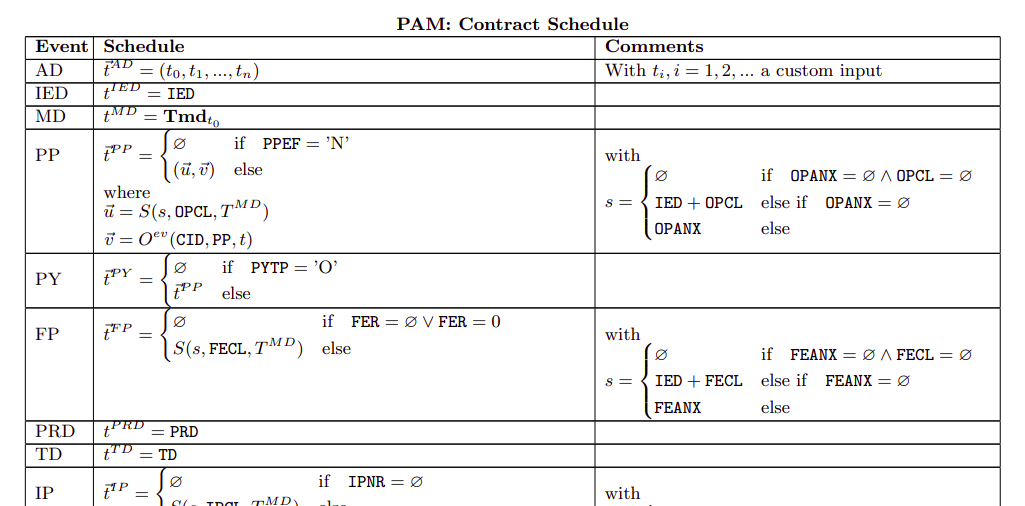
\includegraphics[width=\textwidth]{PAM_Contract_Schedule.png}
    \caption{Cronograma del contrato PAM para algunos eventos}\label{fig:PAM_Contract_Schedule}
\end{figure}

\begin{figure}
    \centering
    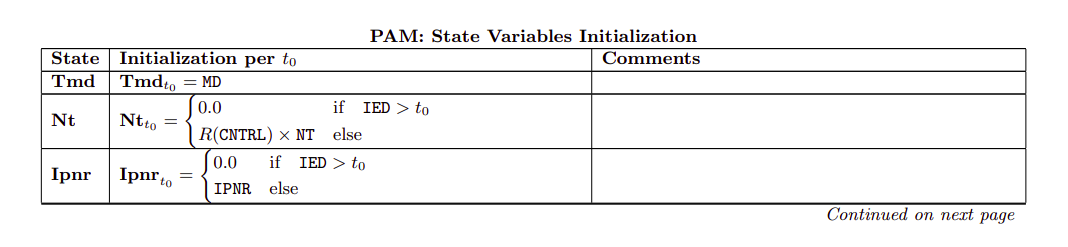
\includegraphics[width=\textwidth]{PAM_State_Variables_Initialization.png}
    \caption{Inicialización de algunas variables del contrato PAM}\label{fig:PAM_State_Variables_Initialization}
\end{figure}

\begin{figure}
    \centering
    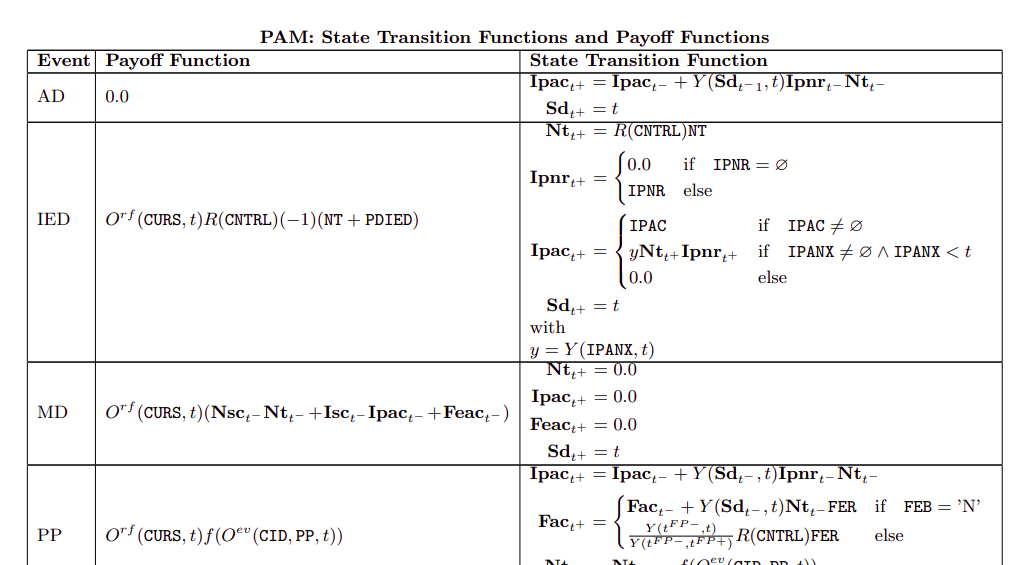
\includegraphics[width=\textwidth]{PAM_STF_POF.png}
    \caption{Funciones de cambio de estado y pago del contrato PAM}\label{fig:PAM_STF_POF}
\end{figure}


%##########################
% Verificación de programas
%##########################

\chapter{Verificación de programas}
\section{Concepto general, herramientas, metodologías}
\section{Isabelle}

%##########################
% Desarrollo: verificación de contratos financieros usando Isabelle
%##########################

\chapter{Desarrollo: verificación de contratos financieros usando Isabelle}
\section{Escritura de contratos ACTUS para Cardano}
\section{sss}
\section{sss}

%##########################
% Conclusión
%##########################

\chapter{Conclusión}

%##########################
% Apéndice
%##########################

\chapter{Apéndice}

%##########################
% Bibliografía
%##########################

\bibliographystyle{apalike}
\bibliography{bibliografia.bib}

\end{document}